\subsection{SCADA}
SCADA stands for supervisory control and data acquisition. A SCADA system is a software-based application utilized within industrial manufacturing that controls an array of hardware components. Furthermore, as the acronym suggests, a SCADA system would contain a data component that would provide a historical overview of a system to the user. Such systems are employed within manufacturing environments in order to consolidate controls over multiple production lines, collect actionable data and to drive business decisions leading to process control and improvement.

The main goals of a SCADA system are listed:
\begin{enumerate}
    \item Control of manufacturing equipment on the plant floor
    \item Control and view of plant floor devices: Programmable Logic Controllers, sensors, valves, variable frequency drives, temperature probes, etc
    \item Display of real-time critical process information
    \item Acquisition, storage, and display of historical data
\end{enumerate}
 
\begin{figure}[H]
    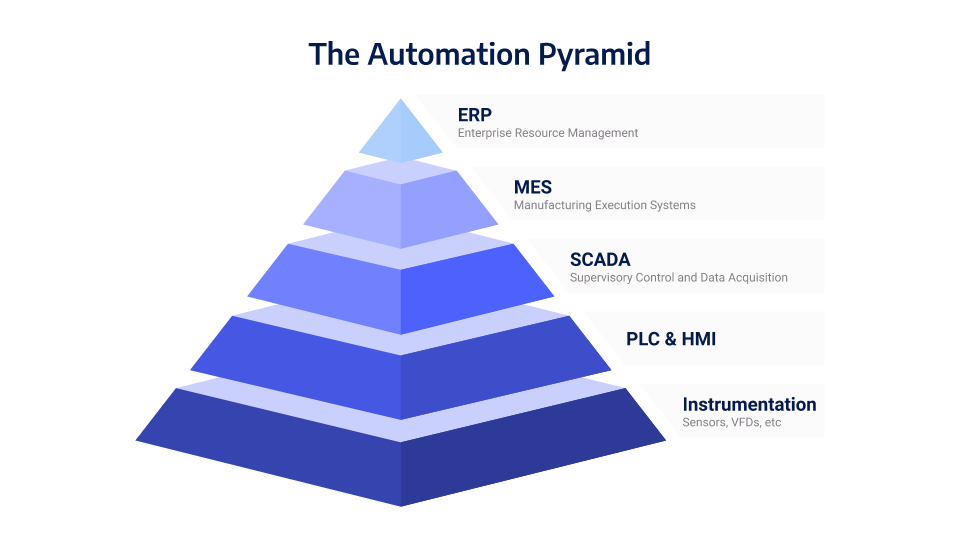
\includegraphics[scale=0.45]{figs/auto_pyramid.png}
    \caption{Automation pyramid to highlight how SCADA fits on here}
\end{figure}
A SCADA system would need to receive information from the PLC \& HMI to communicate with the instrumentation layer. Here PLC stands for programmable logic controller and HMI stands for human machine interface. The HIM system would display the current status of the system, alarms associated with the asset as well as a control screen used to make adjustments. An HMI would send the information to the PLC and vice versa; it would not interact with the instrumentation directly.

\begin{concept}
    Control systems engineers to create a communication layer that would be instantiated within every PLC in order to pass data accordingly. An important infrastructure within this layer is the network. Although the PLC and HMI layers will require a network for data, the SCADA system would create an additional strain on the plant network due to the volume of data it will consume.

    SCADA refers to software while a PLC will refer to hardware. PLC as the brain of the production floor while SCADA connects to the PLC and processes this information.
\end{concept}

\subsubsection{Popular SCADA Software}
Different approaches to different components for each system results in each one being better suited for certain applications

Here are the following softwares mentioned:

Rockwell Automation - FactoryTalk View Site Edition and ThinManager
\begin{itemize}
    \item 
\end{itemize}

Siemens - WinCC RT Professional
\begin{itemize}
    \item 
\end{itemize}

Schneider Electric [AVEVA] - Wonderware
\begin{itemize}
    \item 
\end{itemize}

Inductive Automation - Ignition
\begin{itemize}
    \item 
\end{itemize}
